\documentclass[parskip=half, titlepage=firstiscover, captions=tableheading, bibliography=totoc]{scrartcl}
%optionen immer variieren tabelheading bei tabellen
%ohne parskip nur einrücken
%draft macht hüllen von bilder selbst wenn sie nicht existieren um einfach zeit bei compilieren zu sparen
%\usepackage{scrhack} % nach \documentclass
\usepackage{float}
\floatplacement{figure}{htbp}
\floatplacement{table}{htbp}
\usepackage[aux]{rerunfilecheck}
\usepackage{polyglossia}
\usepackage{biblatex}
\addbibresource{Tag3.bib}%name der bib-Datei hier einfügen !
\setmainlanguage{german}
\usepackage{longtable}
\usepackage{amsmath}
\usepackage{amssymb}
\usepackage{mathtools}
\usepackage{fontspec}
\usepackage[
math-style=ISO,
bold-style=ISO,
sans-style=italic,
nabla=upright,
partial=upright,
]{unicode-math}

\setmathfont{Latin Modern Math}
\usepackage{graphicx}
\usepackage{grffile}
\usepackage[font = scriptsize, labelfont = bf,margin={10pt,10pt}]{subcaption}
\usepackage[font = scriptsize, labelfont = bf,margin={10pt,10pt}]{caption}
%anstatt margin geht auch width = 10cm
\usepackage{mleftright}
%schöneres mit  \mleft (\mright)

\setlength{\delimitershortfall}{-1sp}
%bei vielen Klammern werden sie nun größer
\usepackage[locale=DE,separate-uncertainty=true,per-mode=symbol-or-fraction]{siunitx}
\usepackage{booktabs}
\usepackage{xfrac}
\usepackage{pdflscape}
%-> dazu wäre begin{landscape} etc nötig

%nur ein beispiel zu dieser änderung wenn man will
%gleiche sachen werden bei mathe oder text anders benutzt
%\let\vaccent=\v % alten Befehl kopieren
%\RenewDocumentCommand \v {} % Befehl überschreiben
%{
%\TextOrMath{
%\vaccent % Textmodus
%}{
%\symbf % Mathemodus
%}
%}

%\NewDocumentCommand \OverfullCenter {+m} {
%\noindent\makebox[\linewidth]{#1} }
%bei zu breiten pics zentrierte ausrichtung
%zu befehl wäre dann: \OverfullCenter{\includegraphics[width=\textwidth+15pt]{figures/
%Panorama.jpg}}

\AtBeginDocument{ % wird bei \begin{document} ausgeführt
\let\symIm=\Im % werden sonst wieder von unicode-math überschrieben
\RenewDocumentCommand \Re {}
{
\operatorname{Re}
}
\let\symIm=\Im
\RenewDocumentCommand \Im {}
{
\operatorname{Im}
}
}


\usepackage{fontspec}%nach amssymb
\usepackage[unicode]{hyperref}
\usepackage[shortcuts]{extdash} % nach hyperref, bookmark am Ende!
\usepackage{bookmark}

\title{Protokoll zum Versuch 354:\\ Gedämpfte und erzwungene Schwingungen}
\author{Kyra Klos \and Leonard Borg}
\date{Durchführung: 03.11.2015, Abgabe: 10.11.2015}
\begin{document}
  \maketitle
  \setcounter{tocdepth}{1}
  \tableofcontents
  \newpage
  % !TEX program = lualatex
\documentclass{scrartcl}
\usepackage{amsmath}
\usepackage{amssymb}
\usepackage{unicode-math}
\usepackage{mathtools}
\usepackage{fontspec}
\usepackage{polyglossia}
\begin{document}


    \section{Zielsetung}
    In diesem Versuch werden anhand eines LRC-Schwingkreises die verschieden Lösungen der Schwingungsgleichung untersucht.
    Es werden gemessen: der effektive Widerstand im Fall der homogenen gedämpften Schwingung,
    der Widerstand bei dem der aperiodische Grenzfall eintritt und inhomogenen Fall die Resonanzfrequenz, sowie die Phasenverschiebung,
    die der Schwingkreis verusacht.


    \section{Theorie}
    \subsection{Schwingungsgleichung}
    \label{sub:Schwingungsgleichung}

    \label{sec:Theorie}
    Der gegebene, wie auch der standard LRC-Reihenschwingkreis besteht aus Einer Induktivität L, einem ohmschen Widerstand R und einer Kapazität C.
    Im Idealfall ($R=0$) wird nur zwischen der Induktivität und der Kapazität harmonisch Energie ausgetauscht, ist $R > 0$ so nimmt diese auch exponentiell ab,
    da sie vom Widerstand des Stromkreises in Wärme umgesetzt wird.

    Aus der Maschenregel (2. kirchhoffsches Gesetz) folgt, dass die Summe der Spannungen in einem geschlossenen Stromkreis gleich Null ein müssen, also muss gelten:
    \begin{equation}
        U_L(t)+U_R(t)+U_C(t)=0.
        \label{eqn:Krichhoff2}
    \end{equation}
    Für die gegebenen Spannungen gelten die Identitäten
    \begin{align*}
        U_L &= \dot{I}L \\
        U_R &= IR  \\
        U_C &= \frac{Q}{C}.
    \end{align*}
    Dies ergibt mit $I=\dot{Q}$ die homogene Schwingungsgleichung in I:
    \begin{equation}
        L\ddot{I}+R\dot{I}+\frac{1}{C}I=0
        \label{eqn:Schwingungsgleichung}
    \end{equation}
    Die Lösung für diese DGL lautet
    \begin{equation}
        I(t)=e^{-2\pi\mu t}(A_0e^{2\pi\nu it}+A_1e^{-2\pi\nu it})
        \label{eqn:Fundamentalsys}
    \end{equation}
    mit
    \begin{align}
        \mu &= \frac{R}{4\pi L}\\
        \text{und}\\
        \nu &= \frac{1}{2\pi}\sqrt{\frac{1}{LC}-\frac{R^2}{4L^2}}
    \end{align}

    Der Verlauf der entsprechenden Ladungs- bzw. Spannungskurve hängt nun davon ab,
    ob $\nu$ reelwertig ist oder echt komplexe Werte annimmt:
    \begin{equation*}
        \nu \in \mathbb{R} \iff \frac{1}{LC} > \frac{R^2}{4L^2}.
    \end{equation*}

    Mit $e^{i\phi}= cos(\phi)+isin(\phi)$ und (\ref{eqn:Fundamentalsys}) folgt dann:
    \begin{equation}
        I(t) = e^{-2\pi\mu t}cos(2\pi\nu t)
    \end{equation}
    Die Zeit, zu der Exponent genau -1 ist nennt man Abklingdauer:
    \begin{equation}
        T_{ex} := \frac{1}{2\pi\mu}.
        \label{eqn:Abkling}
    \end{equation}
    Für $\nu = 0$ tritt der sog. aperiodische Grenzfall ein,
    wo $I(t)$ durch nur eine Exponentialfunktion beschrieben werden kann und es somit zu keiner Schwingung kommt.
    In diesem Fall nähert sich die Auslenkung am schnellsten Null von allen Lösungen der DGL.
    \subsubsection{Getriebene Schwingung}
    \label{subs:Getriebene Schwingung}

    Im weitern Verlauf des Versuchs wird ein mit einer Wechselspannung getriebener Schwingkreis
    untersucht. Die Differentialgleichung muss daher um  eine Inhomogenität der Form:
    \begin{equation*}
        U_0e^{i\omega_0 t}
    \end{equation*}
    ergänzt werden.Nachdem sich das System eingeschwungen hat und $\omega =\omega_0$ gilt berechnet sich die Spannung am Schwingkreis mit
    \begin{equation}
        |U(t)| = U_0\sqrt{\frac{(1-LC\omega^2)^2+\omega^2R^2C^2}{((1-LC\omega^2)^2+\omega^2R^2C^2)}}
    \end{equation}
    Mit der komplexen Phase
    \begin{equation}
        \label{eqn:Phase}
        \phi(\omega) = atan\left(\frac{-\omega RC}{1-LC\omega^2}\right).
    \end{equation}
    Da gilt $|U_C|=|U(t)|$, folgt
    \begin{equation}
        U_C(\omega)=\frac{U_0}{\sqrt{(1-LC\omega^2)^2+\omega^2R^2C^2}}
    \end{equation}
    An dieser Formel kann man erkennen, dass gilt
    \begin{align}
    {\omega &= 0 \implies U_C = U_0} ,

    \text{und außerdem, dass für große}
    \omega : U_C &\propto \frac{1}{\omega^2} \rightarrow 0.
    \end{align}
    Für Phasen $\Phi_1,\Phi_2$ bei  $\frac{\pi}{4}$ und $\frac{3}{4} \pi$ respektive gilt:
    \begin{equation}
        \label{eqn:Spektrum}
        \omega_{1,2}=\pm \frac{R}{2L}+\sqrt{\frac{R^2}{4L^2}+\frac{1}{LC}}
    \end{equation}
    Außerdem gilt für die Resonanzfrequenz
    \begin{equation}
        \label{eqn:ResFrequenz}
        \omega_{res} = \sqrt{\frac{1}{LC}-\frac{R^2}{2L^2}} ,
    \end{equation}
    wo der Maximalwer von $U_C(\omega)$ erreicht wird, der i.d.R. deutlich höher ist als U_0.

     Wenn die Dämpfung schwach ist, also gilt
     \begin{equation*}
         \frac{R^2}{2L^2}\ll \frac{1}{LC} ,
     \end{equation*}
     so vereinfacht sich das Problem auf eine ungedämpfte Schwingung, bei der die Eigenfrequenz des Schwingkreises dann gegeben ist durch
     \begin{equation}
         \omega_0 = \sqrt{\frac{1}{LC}} .
     \end{equation}

     Für diesen Fall gilt dann $\omega_{res} \approx \omeaga_0$ und daher
     \begin{equation}
         \label{eqn:Güte}
         U_C(\omega_{res})= qU_0
         \text { mit }
          q=\frac{1}{\omega_0 RC}
     \end{equation}
     Man nennt q dann die Güte des Schwingkreises. Zusätzlich wird gewöhnlich auch die Breite der Resonanzkurve von $U_C(\omega)$ angegeben
     mit der Näherung
     \begin{equation}
         \label{eqn:Breite}
         \omega_+ -\omega_- \approx \frac{R}{L} .
     \end{equation}

\end{document}

  %!TEX program = lualatex
\documentclass{scrartcl}
\usepackage{amsmath}
\usepackage{amssymb}
\usepackage{unicode-math}
\usepackage{mathtools}
\usepackage{fontspec}
\usepackage{polyglossia}



\begin{document}


\section{Fehlerrechnung}
\label{sec:Fehlerrechnung}

Alle Mittelwerte, sofern nicht anders vermerkt werden mit dem arithmetischen Mittel:
\begin{equation}
    \overline{x}  = \frac{1}{N} \sum_{i=1}^N x_i
\end{equation}
berechnet.\\
Der statistische Fehler dieses Wertes wird berechnet mit
\begin{equation}
    \Delta\overline{x} = \frac{1}{\sqrt{N}}\sqrt{\frac{1}{N-1}\sum_{i=1}^N (x_i-\overline{x})^2}}.
\end{equation}
Werden Fehlergrößen zur weiteren Berechnung genutzt, so wird der Fehler im Resultat
mit der Gauß'schen Fehlerfortpflanzung berechnet:
\begin{equation}
\Delta f = \sqrt{\sum_{i=1}^N \left(\frac{\partial f}{\partial x_i}\right)^2(\Del{x_i})}
\end{equation}

Auftretende Ausgleichsgraden werden berechnet nach der linearen Regression mit
\begin{align}
    y &= ax+b\\
    a &= \frac{\overline{xy}-\overline{x}\overline{y}}{\overline{x^2}-\overline{x}^2}\\
    b &= \frac{\overline{x^2}\overline{y}-\overline{y}\overline{xy}}{\overline{x^2}-\overline{x}^2}
\end{align}


\end{document}

  % !TEX program = lualatex
\documentclass{scrartcl}
\usepackage{polyglossia}
\begin{document}


    \section{Durchführung}
    \label{sec:Durchführung}
    Als erstes wird an den gegebenen Schwingkreis mit vorab bekannten Größen L,R,C
    eine Nadelpulsspannung angelegt und parallel zum Kondensator wird ein Oszilloskop angeschlossen.
    Nun stellt man die Frequenz des Nadelpuls' so ein, dass man nach dem jeweiligen Puls Relaxionsverhalten beobachten kann
    (die Spannung sollte mindestens um $\frac{1}{e}$ abgenommen haben).
    Von der enstehenden Abbildung einer gedäpften (Co-)Sinusschwingung wird der Thermodruck genommen,
    und bei den Extrema der Funktion werden jeweils Zeit seit dem Nadelpuls und Amplitude gemessen.

    Um den Grenzwiderstand $R_ap$ für den aperiodischen Grenzfall zu bestimmen wird nun,
    anstatt einem statischen R ein regelbarer Widerstand in den Schwingkreis geschaltet.
    Dieser wird von seinem Maximalwert so weit reduziert, dass sich eine sichtbare Überschwingung ausbildet
    und dann zurück auf eben den Wert eingestellt wo das Oszilloskop das erste mal eindeutig dem relaxionsverhalten eines geladenen Kondensators gleicht
    Der an diesem Punkt abzulesende Widerstand wird notiert.

    Zur Messung des Verhaltens des getriebenen Schwingkreises wird eine Wechselspannung and den Schwingkreis gelegt
    und zum Abgleich auf den zweiten Kanal des Oszilloskops gespeist.
    Als erstes wird die Amplitude der angelegten Wechselspannung aufgenommen
    und im Folgenden wird die Frequenz $\nu$ am Sinusgenerator variiert.
    Es sollte darauf geachtet werden, dass die Messabstände bei stärkeren Änderungen entsprechend kleiner zu wählen sind.

    Als Abschluss wird $\Phi(\omega)$ bestimmt die Phasenverschiebung, die der Schwingkreis aufgrund seiner Impedanz hervorruft.
    Zunächst wird die Erregerfrequenz klein gehalten, sodass die Erregung überwiegt und beide Wellen phasengleich sind
    und justiert das Oszilloskop so, dass bei beiden Wellen die Nulldurchgänge im selben punkt liegen.
    Und nun variiert man wie zuvor die Frequenz und misst die entstehenden Abstände zwischen den Nulldurchgängen.


\end{document}

\section{Auswertung}
\label{sec:Auswertung}
Hier folgt nun die Auswertung des Experiments, das mit Hilfe des Gräts $2$ durchgeführt wurde.
\begin{align*}
 L &= \SI{10,11(3)e-3}{\henry}\\
 C &= \SI{2,098(6)e-9}{\farad}\\
 R_1 &= \SI{48,1(1)}{\ohm}\\
 R_2 &= \SI{509,5(5)}{\ohm}
\end{align*}
Die Plots wurden mit Hilfe des Programs Gnuplot erstellt.
\subsection[underline]{Zeitabhängigkeit der gedämpften Schwinungsamplitude}
Zuerst wurde die abklingenden Amplituden $U_C$ mit dem Fehler $\pm{0,08}$$\si{\volt}$ des LCR-Schwingkreises im Bezug auf
die Zeit $t_i$ mit der Ungenauigkeit von $\pm{2}$$\si{\micro\s}$ gemessen.(Siehe Abbildung 1)
\begin{table}
  \centering
  \caption{Hier sieht man deutlich den exponentiellen Abfall der Ampiltuden der Schwingung mit $\SI{1997}{\hertz}$ Eregerfrequenz zu der Zeit}
  \label{tab:Daten1}
  \begin{tabular}{S S}
   \toprule
   {$U_C\:/\:\si{\volt}$} & {$t_i\:/\:\si{\micro\sec}$} \\
   \midrule
  4,56 & 12\\
  3,76 & 28\\
  3,36 & 44\\
  2,64 & 56\\
  2,40 & 70\\
  2,24 & 86\\
  1,76 & 102\\
  1,60 & 116\\
  1,36 & 128\\
  1,20 & 146\\
  0,96 & 158\\
  0,96 & 173\\
  0,80 & 186\\
  0,72 & 202\\
  0,56 & 216\\
  0,56 & 230\\
  0,48 & 240\\
   \bottomrule
  \end{tabular}
 \end{table}
Besonders hervor zu heben ist der Dämpfungswiderstand des aperiodischen Grenzfalls,der experimentel einen Wert von $\SI{3,19(1)}{\kilo\ohm}$ beträgt.
Verglichen mit dem durch ($ R = \sqrt{4L/C}$) errechneten Widerstand von $\SI{4,39(9)}{\kilo\ohm}$, ist eine Differenz von ~ $\SI{1,4}{\kilo\ohm}$ zu ersehen.
Durch die Ausgleichrechnung erhält man $\mu$ aus dem Exponenten der Gleichung (6) und kann somit durch (4 und 7) folgendes berechnen:
\begin{align*}
 T_{ex} &= \SI{93,2(1)}{\micro\s}\\
 R_{eff} &= \SI{216,9(5)}{\ohm}
\end{align*}
Vergleicht man nun den effektiven Widerstand $R_{eff}$ mit dem in der Schaltung eingesetzten von $\SI{48,1(1)}{\ohm}$ , ist eine deutliche Diskrepanz von ungefähr $\SI{150}{\ohm}$ zu erkennen.
\begin{figure}
\centering
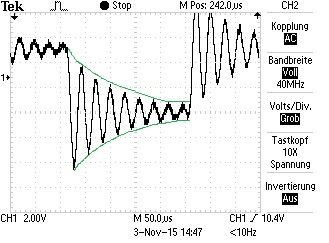
\includegraphics{Thermo.jpg}
\caption{Thermodruck des zeitlichen Abklingens der gedämpften Schwingungsamplitude\\ mit der Einfüllenden(in grün).}
\label{fig:thermodruck}
\end{figure}
\newpage
\subsection[underline]{Messung der Frequenzabhängigkeiten an einem LCR-Schwingkreis}
In der folgenden Tabelle sind die Daten aus der Messreihe der Kondensatorspannung  mit der Ungenauigkeit $\pm{0,3}$$\si{\volt}$ zu den Frequenzenmit mit der Ungenauigkeit $\pm{0,03}$$\si{\kilo\hertz}$, sowie das Verhältnis dieser zur Eregerspannung von ca. $\SI{10}{\volt}$ zu finden.
Diese Daten sind in zwei Plots einem in linear (Abbildung 2) und einem in halblogarithmischer (Abbildung 3) Form aufgetragen.
Wichtig hierbei zu erwähnen ist,dass ab einschließlich dem Wert $\SI{27,15}{\kilo\hertz}$ die Skala vergrößert wurde, sodass sich die darauffolgenden Werte leicht verschieben können.
Aus dem Linearen (Abbildung 2) der darauffolgenden Plots, in dem die Frequenz zum Spannungsverhältnis aufgetragen wurde, sind die experimentellen Werte für die Resonanzüberhöhung bzw. Güte q, sowie die Breite der Resonanzkurve $\nu_1 - \nu_2$ entnommem und werden hier mit den durch (14 und 15) berechneten Werten mit einem Gesamtwiderstand von $\SI{559,5(5)}{\ohm}$ verglichen:
\begin{align*}
q_{theo} &= \si{3,923(5)} & q_{exp} &= \si{3,72}\\
\text{Theoretisch:} \symup{\nu_+} - \symup{\nu_-} &= \SI{8,81(3)e3}{\hertz} & \text{Experimentell:} \symup{\nu_+} - \symup{\nu_-} &= \SI{11,19e3}{\hertz}
\end{align*}
Die realtiv gerringen Differnezen von q bei etwa $0,2$ und bei Resonanzkurvenbreite bei etwa $\SI{1,3e3}{\ohm}$ sind im Fehlertolerenazbereich und benötigen somit keine weitere Erläuterung.
\begin{table}
  \centering
  \caption{Die Messdaten zeigen hierbei einen deutlichen Anstieg bis zum Maximum, sowie eine nachträglichen Abfall gleichermaßen}
  \label{tab:Daten2.1}
  \begin{tabular}{S S S}
    \toprule
    \multicolumn{1}{c}{$\si{\nu}\:/\:\si{\kilo\hertz}$} & \multicolumn{1}{c}{$U_C\:/\:\si{\volt}$} & \multicolumn{1}{c}{$U_C/U$}\\
    \midrule
    2,00 & 10,0 & 1,00\\
    4,00 & 10,0 & 1,00\\
    5,00 & 10,2 & 1,02\\
    7,50 & 10,4 & 1,04\\
    9,00 & 10,6 & 1,06\\
   11,00 & 11,0 & 1,10\\
   14,00 & 11,5 & 1,15\\
   16,00 & 12,0 & 1,20\\
   18,00 & 12,6 & 1,26\\
   18,65 & 13,0 & 1,30\\
   19,50 & 13,6 & 1,36\\
   20,30 & 14,0 & 1,40\\
   21,00 & 14,6 & 1,46\\
   21,45 & 15,0 & 1,50\\
   22,50 & 15,8 & 1,58\\
   23,00 & 16,3 & 1,63\\
   23,60 & 16,9 & 1,69\\
   24,20 & 17,6 & 1,76\\
   24,55 & 18,0 & 1,80\\
   25,00 & 18,6 & 1,86\\
   25,35 & 19,0 & 1,90\\
   25,65 & 19,4 & 1,94\\
   26,10 & 20,1 & 2,01\\
   26,50 & 20,7 & 2,07\\
   26,80 & 21,2 & 2,12\\
   27,10 & 21,7 & 2,17\\
   27,15 & 22,4 & 2,24\\
   27,50 & 22,8 & 2,28\\
   28,00 & 24,0 & 2,40\\
   28,40 & 24,8 & 2,48\\
   28,60 & 25,2 & 2,52\\
   29,05 & 26,4 & 2,64\\
   29,35 & 27,2 & 2,72\\
   29,50 & 27,6 & 2,76\\
   29,85 & 28,4 & 2,84\\
   30,00 & 28,8 & 2,88\\
   30,15 & 29,2 & 2,92\\
  \bottomrule
\end{tabular}
\end{table}
\begin{table}
  \centering
  \label{tab:Daten2.2}
  \begin{tabular}{S S S}
  \toprule
    \multicolumn{1}{c}{$\si{\nu}\:/\:\si{\kilo\hertz}$} & \multicolumn{1}{c}{$U_C\:/\:\si{\volt}$} & \multicolumn{1}{c}{$U_C/U$}\\
  \midrule
   30,25 & 29,6 & 2,96\\
   30,45 & 30,0 & 3,00\\
   30,55 & 30,4 & 3,04\\
   30,70 & 30,8 & 3,08\\
   30,85 & 31,2 & 3,12\\
   31,00 & 31,6 & 3,16\\
   31,10 & 32,0 & 3,20\\
   31,25 & 32,4 & 3,24\\
   31,55 & 33,4 & 3,34\\
   31,70 & 33,2 & 3,32\\
   31,90 & 34,0 & 3,40\\
   32,20 & 34,8 & 3,48\\
   32,35 & 35,2 & 3,52\\
   32,55 & 35,6 & 3,56\\
   32,80 & 36,0 & 3,60\\
   33,35 & 36,8 & 3,68\\
   34,00 & 37,2 & 3,72\\
   34,50 & 36,8 & 3,68\\
   35,00 & 36,4 & 3,64\\
   35,50 & 35,2 & 3,52\\
   36,00 & 33,6 & 3,36\\
   36,50 & 32,3 & 3,23\\
   37,00 & 30,6 & 3,06\\
   37,50 & 29,0 & 2,90\\
   38,00 & 27,2 & 2,72\\
   38,50 & 25,6 & 2,56\\
   39,00 & 24,0 & 2,40\\
   39,50 & 22,4 & 2,24\\
   40,00 & 21,2 & 2,12\\
   41,00 & 19,0 & 1,90\\
   42,00 & 16,8 & 1,68\\
   43,00 & 15,2 & 1,52\\
   44,00 & 14,0 & 1,40\\
   45,00 & 12,8 & 1,28\\
   46,00 & 11,6 & 1,16\\
   47,00 & 10,8 & 1,08\\
   48,00 & 10,0 & 1,00\\
   49,00 & 9,2 & 0,92\\
   50,00 & 8,6 & 0,86\\
   55,00 & 6,4 & 0,64\\
\bottomrule
\end{tabular}
\end{table}
\begin{figure}
  \centering
  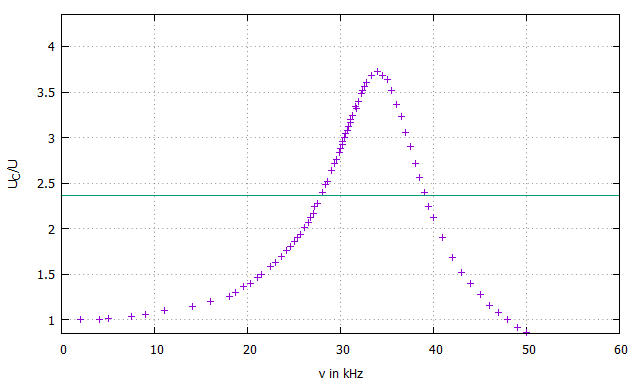
\includegraphics[width=\textwidth]{Linear1.jpeg}
\caption{Aus der hierzusehenden linearen Darstellung der Freuquenzabhänigkeit der Spannung \\ sind die Daten zur Güte und die Resonanzkurve mit ihren eingezeichten Ränder anzulesen.}
\label{fig:Linear1}
\end{figure}
\begin{figure}
  \centering
  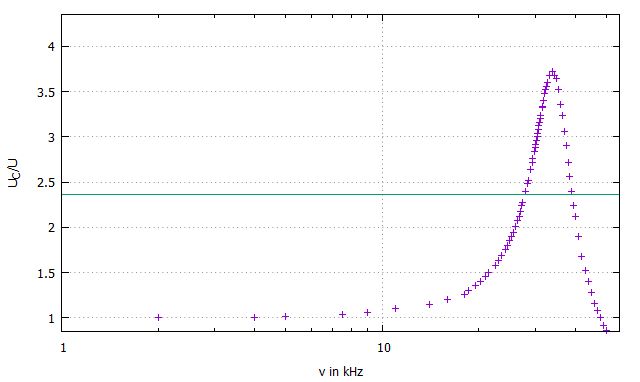
\includegraphics[width=\textwidth]{Halblog1.jpeg}
  \caption{Hier ist die halblogarithmische Darstellung des Spannungs-Frequenzverhältnisses zu sehen.}
  \label{fig:Halb1}
\end{figure}

\subsection[underline]{Messung der Phasen zwischen Erreger- und Kondensatorspannung}
Im letzten Teil des Experiments wurden die Phasendifferenzen $\delta$t zu den einzelnen Frquenzen gemessen und daraus die Pahsenverschiebuung $\varphi$ im Bogenmaß berechnet.
Hier sind die Phasenverschiebung $\varphi$ und die Phasendifferenz $\delta$t mit der Ungenauigkeit $\pm{0,2}$$\si{\micro\s}$ zur Frequenz $\nu$ vom Verhälnis LCR-Schwingkreis zu Sinus-Schwingungsgenerator.
\begin{table}
  \centering
  \caption{Hier sieht man die Werte, der durch Lissajou-Figuren gemessenen Phasendifferenz, und die dazugehörige Verschiebung zu den Frequenzen.}
  \label{tab:Daten3}
  \begin{tabular}{S S S}
    \toprule
    \multicolumn{1}{c}{$\symup{\nu}\:/\:\si{\kilo\hertz}$} & \multicolumn{1}{c}{$\symup{\Delta}t\:/\:\si{\micro\sec}$} & \multicolumn{1}{c}{$\symup{\varphi}\:/\:rad$}\\
    \midrule
    2,0 & 0,00 & 0,0000 \\
    5,0 & 1,00 & 0,0314 \\
   10,0 & 1,00 & 0,0628 \\
   15,0 & 1,50 & 0,1414 \\
   20,0 & 1,80 & 0,2262 \\
   25,0 & 2,10 & 0,3300 \\
   27,5 & 3,00 & 0,5184 \\
   30,0 & 4,00 & 0,7540 \\
   30,5 & 4,10 & 0,7854 \\
   31,0 & 4,50 & 0,8765 \\
   32,0 & 5,20 & 1,0455 \\
   33,0 & 6,00 & 1,2440 \\
   33,5 & 6,50 & 1,3681 \\
   34,0 & 6,70 & 1,4313 \\
   34,5 & 7,50 & 1,6258 \\
   35,0 & 7,50 & 1,6493 \\
   35,5 & 8,00 & 1,7844 \\
   36,0 & 8,50 & 1,9227 \\
   36,5 & 8,70 & 1,9952 \\
   37,0 & 9,00 & 2,0923 \\
   37,5 & 9,25 & 2,1795 \\
   38,0 & 9,50 & 2,2682 \\
   38,5 & 9,50 & 2,2980 \\
   39,0 & 9,50 & 2,3279 \\
   39,5 & 9,75 & 2,4198 \\
   40,0 & 9,75 & 2,4504 \\
   \bottomrule
 \end{tabular}
 \end{table}

Die Plots der Frequenzen in Abhängigkeit der Phasenverschiebung sind in halblogarithmischer (Abbildung 5) und linearer (Abbildung 4) Form in den folgenden Abbildungen zusehen.\\
Aus Letztrem werden die experimentellen Werte für die Resonanzspannung $\nu_res$ , die sich im Bereich von $\pi/2$ befindet, sowie die Ränder der Resonanzkurve $\nu_1$ und $\nu_2$ bei $\pi/4$ und $3*\pi/2$ entnommen.
\begin{figure}
  \centering
  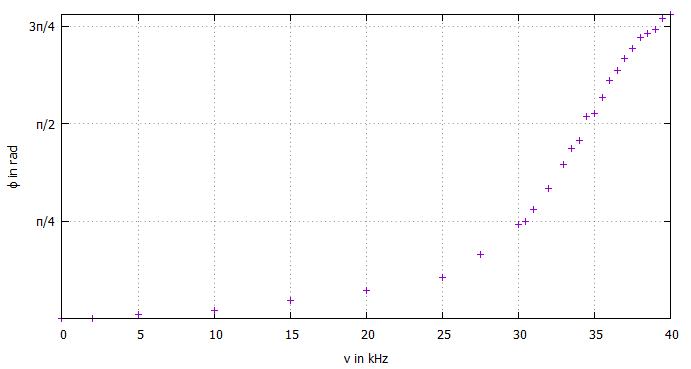
\includegraphics[width=\textwidth]{Linear2.jpeg}
  \caption{Die lineare Darstellung des Verhältnisses Phasenverschiebung von Erreger- und Kondensatorspannung zur Frequenz.}
  \label{fig:Linear2}
\end{figure}
Hier in der linearen Abbildung ist gut der extreme Antsieg der arctan-annäherden Kurve zu sehen.\\Die Spitze und ihr Abflachen sind, durch die begrentzte Maximalfrequenz nur zu erahnen.
\begin{figure}
  \centering
  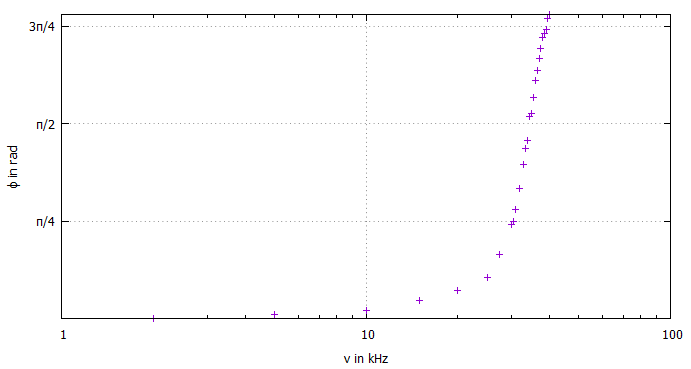
\includegraphics[width=\textwidth]{Halblog2.jpeg}
  \caption{Die halblogarithmische Darstellung der Ferquenzabhängigkeit der Phase zwischen Erreger- und Kondensatorspannung.}
  \label{fig:Halb2}
\end{figure}
\newpage
Die experimentellen Werte werden mit den durch (12) für die Resonanzspannung und (11) für die Ränder der Resonanzkurve berechneten Werten verglichen:
\begin{align*}
  \text{Theoretisch:}\nu_{res} &= \SI{34,55(8)}{\kilo\hertz} & \nu_1 &= \SI{30,78(4)}{\kilo\hertz} & \nu_2 &= \SI{38,80(3)}{\kilo\hertz}\\
  \text{Experimentell:}\nu_{res} &= \SI{34,60}{\kilo\hertz} & \nu_1 &= \SI{30,50}{\kilo\hertz} & \nu_2 &= \SI{39,0}{\kilo\hertz}
\end{align*}
\input{Disskusion.tex}
\newpage
\input{Literatur.tex}
 \end{document}
